\documentclass{article}
\usepackage{mathnotes}

\title{Groups}
\description{Mathematical groups and their fundamental properties including closure, associativity, identity, and inverse elements.}

\begin{document}

\section{Groups}

\subsection{Definition}

\begin{definition}[group]
A group is a set $G$ together with a binary operation $\*$ such that:

\textbf{Closure}: The set is closed under the binary operation. For all $a, b \in G, a \* b \in G$.

\textbf{Associativity}: The binary operation is associative on the set. For all $a, b, c \in G, (a \* b) \* c = a \* (b \* c)$.

\textbf{Identity}: The set contains an identity element, denoted $e$. For all $a \in G, a \* e = a$.

\textbf{Inverses}: All elements in the set have inverse elements in the set, denoted using $a^{-1}$. For all $a \in G$ there exists $a^{-1} \in G$ such that $a \* a^{-1} = e$.

This set/operation combination $G$ is commonly denoted as the pair $(G, \*)$.
\end{definition}

\subsection{Examples}

\begin{example}[Examples of Groups]
Some examples of \dref{groups}:

\begin{itemize}
\item The integers under addition: $(\mathbb{Z}, +)$. The identity element is $0$.
\end{itemize}

\begin{itemize}
\item The non-zero reals under multiplication: $(\mathbb{R}^{\*}, \*)$. The identity element is $1$.
\end{itemize}

\begin{itemize}
\item $n \times n$ invertible matrices.
\end{itemize}

\href{https://en.wikipedia.org/wiki/Examples_of_groups}{Loads more listed here}.

A non-example is the naturals under addition - $(\mathbb{N}, +)$. The naturals are closed under addition, but there is no identity element since $0$ isn't included, and thus no inverses either.
\end{example}

\subsection{Abelian Groups}

\begin{definition}[Abelian]
Abelian groups are groups whose operation is commutative. For $a,b \in G, a \* b = b \* a$.
\end{definition}

\begin{example}[Abelian and Non-Abelian Groups]\label{abelian-examples}
The integers under addition are \dref{Abelian}, because $a + b = b + a$, but invertible $n \times n$ matrices are not, because it's not necessary that $AB = BA$.
\end{example}

\subsection{Finite Groups}

The examples given so far are all infinite groups, but finite groups also exist.

\begin{example}[A Finite Group]\label{z4-finite-group}
$(Z_4, +_4)$ i.e. $\{0, 1, 2, 3\}$ together with addition mod $4$ is a finite group.
\end{example}

\subsection{Subgroups}

\begin{definition}[subgroup]
A subgroup $H$ of a group $G$ is a subset of $G$ together with the same operation as $G$ that still forms a group. The identity element of $G$ must also be the identity element of $H$.
\end{definition}

\begin{example}[Even Integers as a Subgroup]\label{even-integers-subgroup}
The even integers under addition, $(2\mathbb{Z}, +)$, are a \dref{subgroup} of the integers under addition.
\end{example}

\begin{definition}[normal]
A subgroup $H$ of a group $G$ is normal if its left and right cosets coincide, that is, if $gH = Hg$, i.e. $gHg^{-1} = H$, for all $g \in G$.
\end{definition}

\subsection{Cyclic Groups}

\begin{definition}[cyclic group]
A \textbf{cyclic group} is a group where there exists some $g \in G$ such that every element in $G$ can be generated from the group operation applied to $g$.

That is, $G = \{g^n | n \in \mathbb{Z}\}$ when we think of the operation as multiplication, or $G = \{ng | n \in \mathbb{Z}\}$ when we think of the operation as addition.
\end{definition}

\begin{note}[Generator Notation]
We use angle brackets to denote an element as a generator. For example, $\langle 1 \rangle$ is a generator of $(\mathbb{Z}, +)$, because every integer can be written as $n1$ for some $n \in \mathbb{Z}$.
\end{note}

\begin{definition}[order]
The \textbf{order} of a finite group is the number of its elements. The order of group $G$ is denoted as $\ord{(G)}$ or $\|G\|$. The order of an element $a$ (also called period length or period) is the number of elements in the subgroup generated by $a$, and is denoted by $\ord{(a)}$ or $\|a\|$.
\end{definition}

\subsubsection{Cyclic Subgroups}

\begin{definition}[cyclic subgroup]
Any subgroup of a cyclic group is also cyclic - a cyclic subgroup.
\end{definition}

\begin{theorem}\label{cyclic-subgroup-generated-by-powers}
Let $G = \langle a \rangle$ be a cyclic group with $n$ elements. Let $b \in G$ and $b = a^s$. Then $b$ generates a cyclic subgroup of $G$ containing $\frac{n}{d}$ elements, where $d = \gcd(s, n)$. Two cyclic subgroups $\langle a^s \rangle$ and $\langle a^t \rangle$ are equal if and only if $\gcd(s,n) = \gcd(t, n)$.
\end{theorem}

\begin{proof}
Suppose $g \in G$ with $\ord(g) = n$ and let $m \in \mathbb{N}$. Then, $\langle g^m \rangle = \langle g^{\gcd{(m,n)}} \rangle$.

So, $ \langle g \rangle = \langle g^m \rangle \iff \gcd{(m,n)} = 1$.
\end{proof}

\detach

\begin{note}[Finding the Subgroups of a Cyclic Group]
Every element of a cyclic finite group will generate a \dref{cyclic-subgroup}. Some of these subgroups will be equivalent to others - we denote each subgroup $\langle g^s \rangle$, where $s$ is the smallest natural number that generates the subgroup.

To find the subgroups of a cyclic group, we follow this algorithm, keeping track of which elements we've found the generated subgroup for.

\begin{enumerate}
\item Some element $g$ will generate the entire group. If the group's \dref{order} is $n$, then any element of the form $g^s$ where $s$ and $n$ are relatively prime will also generate the entire group, so note that we've found the generated subgroup for all of those elements.
\end{enumerate}

\begin{enumerate}
\item Starting with the next $g^s$ not covered already, find the subgroup generated by it - all elements of $G$ of the form $(g^s)^k$. Note the order of this subgroup and call it $t$. Any elements of $G$ of the form $r \cdot g^s$ where $r$ is relatively prime with $t$ will generate the same subgroup. Note that we've found the generated subgroup for all of those elements.
\end{enumerate}

\begin{enumerate}
\item Repeat step 2 until we've found the subgroup generated by all elements.
\end{enumerate}
\end{note}

\begin{example}[Subgroups of $Z_{20}$]
This sounds really abstract, so here's an example of finding all of the subgroups of $(Z_{20}, +_{20})$

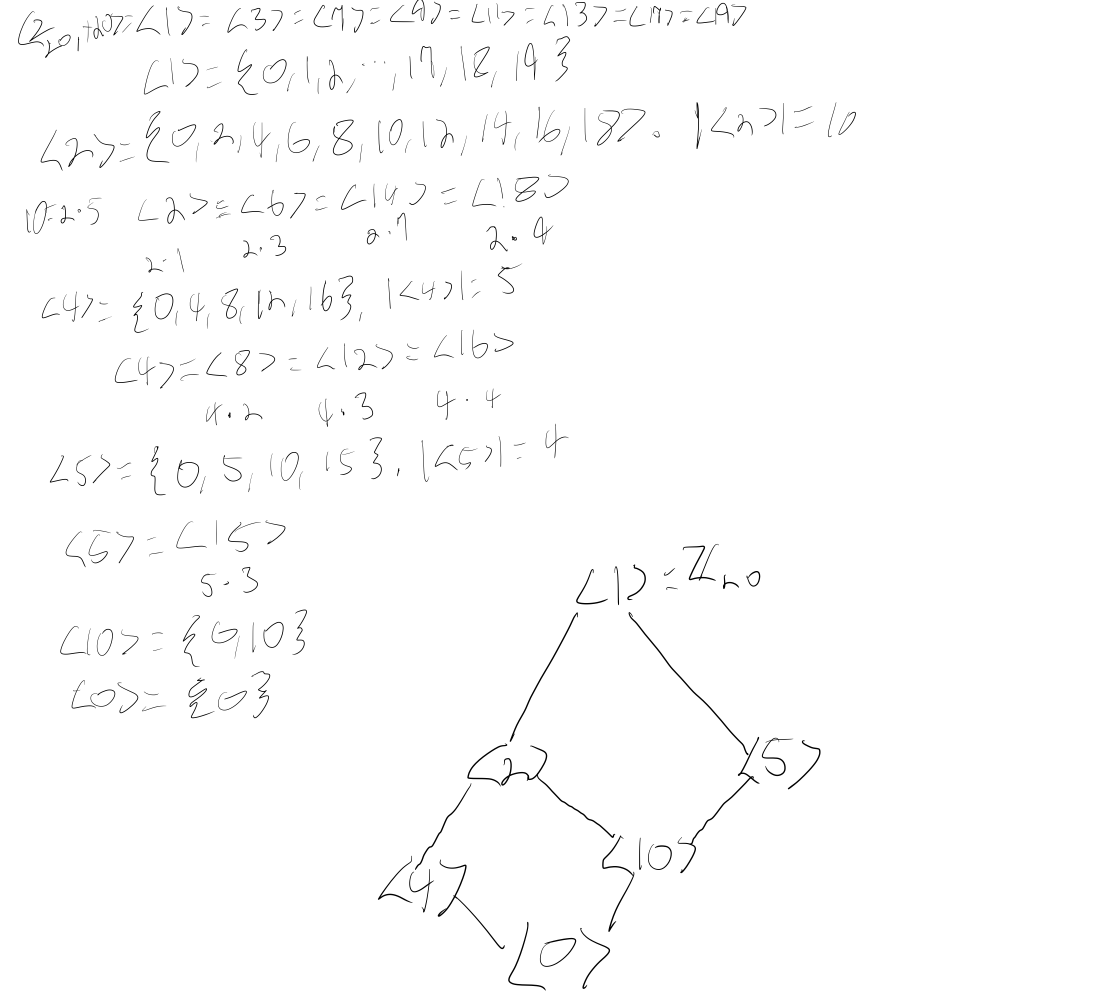
\includegraphics[alt={Cyclic Subgroups of $Z_{20}$}]{subgroupsofZ_20.png}

The diagram in this image is called a subgroup diagram or subgroup lattice. It represents containment - so a node being higher on the diagram indicates that any nodes below it are subsets of it.
\end{example}

\subsection{Permutations}

\begin{example}[Permutation Matrix Notation]
If we rearrange the ordered set $A = \{1,2,3,4,5\}$ to another order, say $\{3,2,5,1,4\}$, then we get a \dref{permutation} of $A$.

This rearrangement is a bijection from $A$ to $A$ that performs

\[ \begin{align} 1 \to 3 \\ 2 \to 2 \\ 3 \to 5 \\ 4 \to 1 \\ 5 \to 4 \end{align} \]

We can represent this permutation compactly using a matrix

\[ \begin{pmatrix} 1 & 2 & 3 & 4 & 5 \\ 3 & 2 & 5 & 1 & 4 \end{pmatrix} \]

Here, the top row is the input and the bottom row is the output, column-wise.
\end{example}

\begin{definition}[permutation]
A permutation is a bijection $\phi : A \to A$, that is, a bijection from a set onto itself.
\end{definition}

\begin{note}\label{permutations-usually-finite}
Generally, we talk about permutations on finite sets, but this doesn't seem to be a hard and fast rule.
\end{note}

The set of all permutations on the set $A$ is denoted by $S_A$:

\[ S_A = \{ \phi : A \to A | \phi \text{ is a bijection} \} \]

\begin{definition}[symmetric group]
When $A$ is the finite set $\{1, 2, 3, \cdots, n\},$ the group of all \dref{permutations} of $A$ is the \textbf{symmetric group} on $n$ letters, and is denoted by $S_n$. It has $n!$ elements.
\end{definition}

\begin{definition}[permutation multiplication]
\dref{Permutations} can be "multiplied", which is just composition. So if we have two permutations on $A$, called $\sigma$ and $\tau$, $\sigma \tau$ means their multiplication, and we apply from right to left, so $\tau$ applies first and then $\sigma$. The result will also be a permutation in $A$.
\end{definition}

Permutation multiplication of permutations of a set forms a group:

\begin{theorem}\label{permutations-form-group}
Let $A$ be a nonempty set, and $S_A$ be the collection of all permutations of $A$. Then $S_A$ is a group under permutation multiplication.
\end{theorem}

\subsubsection{Orbits}

\begin{definition}[orbit containing a point]
Let $\sigma$ be a \dref{permutation} of $A$, the orbit of $\sigma$ containing $a \in A$ is the set

\[ \{ \cdots, \sigma^{-2}(a), \sigma^{-1}(a), a, \sigma{(a)}, \sigma^{2}(a), \cdots \} = \{\sigma^n(a) | n \in \mathbb{Z}\}. \]

So, $a,b \in A$ are in the same orbit of $\sigma$, written as $a \sim b$, if and only if $b = \sigma^n(a)$ for some $n \in \mathbb{Z}$.

The relation "\textasciitilde{}" is an equivalence relation (reflexive, symmetric, transitive). This means $A$ can be partitioned into orbits of $\sigma$.
\end{definition}

\begin{definition}[orbit]
Let $\sigma$ be a \dref{permutation} of $A$. The equivalence classes in $A$ determined by the equivalence relation "\textasciitilde{}" are the \textbf{orbits} of $\sigma$.
\end{definition}

\begin{example}[Orbits of a Permutation in $S_8$]
Consider $\sigma = \begin{pmatrix} 1 & 2 & 3 & 4 & 5 & 6 & 7 & 8 \\\ 3 & 8 & 6 & 7 & 4 & 1 & 5 & 2 \end{pmatrix}$ in $S_8$. The orbit of $\sigma$

\begin{itemize}
\item containing 1 is $\{1,3,6\}$ because $\sigma(1) = 3$, $\sigma(3) = 6$, and $\sigma(6) = 1$.
\end{itemize}

\begin{itemize}
\item containing 2 is $\{2,8\}$.
\end{itemize}

\begin{itemize}
\item containing 4 is $\{4, 5, 7\}$.
\end{itemize}

So the orbits of $\sigma$ are $\{1,3,6\}, \{2,8\}, \{4,5,7\}$.
\end{example}

\subsubsection{Cycles}

\begin{definition}[cycle]
A permutation $\sigma \in S_n$ is a \textbf{cycle} if it has at most one \dref{orbit} containing more than one element. The length of a cycle is the number of elements in its largest orbit.
\end{definition}

\begin{definition}[cyclic notation]
A \dref{cycle} in $S_n$ may be written as $(a_1, a_2, \cdots, a_k)$ - this is called \textbf{cyclic notation}. It represents the permutation that sends $a_1 \to a_2 \to \cdots \to a_k \to a_1$.
\end{definition}

\begin{definition}[disjoint (cycle)]
Two or more cycles are \textbf{disjoint} if no element appears in more than one cycle.
\end{definition}

\begin{theorem}\label{permutation-as-product-of-disjoint-cycles}
Every permutation $\sigma$ of a finite set is a product of disjoint cycles.
\end{theorem}

\subsubsection{Even and Odd Permutations}

\begin{definition}[transposition]
A cycle of length 2 is a \textbf{transposition}.
\end{definition}

\begin{definition}[even (permutation)]
A permutation of a finite set is \textbf{even} if it is the product of an even number of transpositions.
\end{definition}

\begin{definition}[odd (permutation)]
A permutation of a finite set is odd if it is the product of an odd number of transpositions.
\end{definition}

\begin{theorem}\label{permutation-parity-is-well-defined}
A permutation in $S_n$ can be written as either a product of an odd number of transpositions or a product of an even number of transpositions, but not both.
\end{theorem}

\begin{definition}[alternating group]
The subgroup of $S_n$ consisting of all even permutations of $n$ letters is the \textbf{alternating group} $A_n$ on $n$ letters. If $n \geq 2$, then this set forms a subgroup of $S_n$ of order $n!/2$.
\end{definition}

\subsubsection{Cosets}

\begin{definition}[coset]
Let $H$ be a subgroup of $G$. Given $a \in G$, the subset $aH = \{ah | h \in H\}$ of $G$ is the \textbf{left coset} of $H$ containing $a$, while the subset $Ha = \{ha | h \in H\}$ is the \textbf{right coset} of $H$ containing $a$.
\end{definition}

\begin{example}[Left Cosets of $3\mathbb{Z}$]
Left \dref{cosets} of \dref{subgroup} $3\mathbb{Z}$ of $\mathbb{Z}$:

\[ \begin{align} 0 + 3\mathbb{Z} = \{\dots, -9, -6, 0, 3, 6, 9, \dots\} \\ 1 + 3\mathbb{Z} = \{\dots, -8, -5, 1, 4, 7, 10, \dots\} \\  2 + 3\mathbb{Z} = \{\dots, -7, -4, 2, 5, 8, 11, \dots\} \\  \end{align} \]
\end{example}

\begin{proposition}[Properties of Cosets]\label{coset-properties}
\begin{itemize}
\item If $aH \cap bH \neq \emptyset $, then $aH = bH$. This means we can partition $G$ into left \dref{cosets} of $H$.
\end{itemize}

\begin{itemize}
\item If $G$ is \dref{Abelian}, the left cosets and right cosets of $H$ will be equal. So, in the example above, $a + 3\mathbb{Z} = 3\mathbb{Z} + a$.
\end{itemize}

\begin{itemize}
\item The \dref{order} of $aH$ is the order of $H$, that is, $\|aH\| = \|H\|$. Thus, cosets of a subgroup are of equal size.
\end{itemize}
\end{proposition}

\begin{definition}[index]
The number of left cosets of a subgroup $H$ in a group $G$ is the \textbf{index}  $(G:H)$ of $H$ in $G$.
\end{definition}

From the example above, the index of $3\mathbb{Z}$ in $\mathbb{Z}$ is $3$ since there are 3 left cosets.

\paragraph{Layered Cosets}

Here's a proof from a homework exercise I did.

\begin{theorem}\label{lagrange-theorem-for-indices}
Suppose $H$ and $K$ are subgroups of a group $G$ such that $K \leq H \leq G,$ and suppose that $(H : K)$ and $(G : H)$ are both finite. Then $(G : K) = (G: H)(H :K)$ is finite.
\end{theorem}

\begin{intuition}
The intuition here is that each coset of $H$ can be partitioned into $(H:K)$ cosets of $K$, and that $G$ can be partitioned into $(G:H)$ cosets of $H$, so $G$ can be partitioned into $(G:K) = (G:H)(H:K)$ cosets of $K$. Since both $(G:H)$ and $(H:K)$ are given as finite, their product is also finite.
\end{intuition}

\begin{proof}
In more detail, say $G$ can be partitioned into $n = (G:H)$ cosets of $H$, where $n$ is a natural number. Let $A$ be a set of coset representatives $A \subseteq G$ such that $\mathcal{P} = \bigcup_{a_i \in A} a_i H$ is a partition of $G$ formed by the left cosets of $H$.

Then, $\mathcal{P}$ is 

\[ \begin{align} \mathcal{P} = \{ & a_1 H,  \\ & a_2 H, \\ & a_3 H, \\ & \cdots, \\ & a_n H\} \end{align}, \tag{a} \]

and each $a_i H$ is a disjoint coset of $H$ in $G$.

Now, $H$ can be partitioned into $m = (H:K)$ cosets of $K$, where $m$ is a natural number. Let $B$ be a set of coset representatives $B \subseteq H$ such that $\mathcal{Q} = \bigcup_{b_i \in B} b_i K$ is a partition of $H$ formed by the left cosets of $K$.
  
Then, $\mathcal{Q} = \{ b_1 K, b_2 K, b_3 K, \cdots,  b_m K\}$. Now, we can recover $H$ by taking the union of the elements of $\mathcal{Q}$, that is, $H = \bigcup_{q \in \mathcal{Q}} q$, so the elements of $\mathcal{Q}$, after a round of flattening, are the same as those of $H.$ If we replace $H$ in (a) with $\mathcal{Q}$, distribute each $a_n$ group action over the elements of $\mathcal{Q}$, and then take the union across each resulting set we end up with

\[ \begin{align} \mathcal{R} = \{ & a_1 b_1 K, a_1 b_2 K, a_1 b_3 K, \cdots, a_1 b_m K,  \\ 
                                  & a_2 b_1 K, a_2 b_2 K, a_2 b_3 K, \cdots, a_2 b_m K,  \\
                                  & a_3 b_1 K, a_3 b_2 K, a_3 b_3 K, \cdots, a_3 b_m K,  \\
                                  & \cdots, \\
                                  & a_n b_1 K, a_n b_2 K, a_n b_3 K, \cdots, a_n b_m K\}, \end{align} \]

which is $G$ partitioned into the left cosets of $K$. Because we constructed each element in $\mathcal{R}$ by partitioning the elements of a partition of $G$ into cosets of $K$ (then taking their union), we know they are disjoint and cover all of $G$. There are $nm = (G:H)(H:K) = (G:K)$ elements in $\mathcal{R}$, and since $n$ and $m$ are finite, so is $(G:K)$.
\end{proof}

\subsection{Homomorphisms}

\begin{definition}[homomorphism (group)]
A \textbf{homomorphism} is a map $\phi : G \to G'$ between groups (not necessarily a bijection), $\langle G, * \rangle$ and $\langle G', *' \rangle,$ that satisfies the homomorphism property:

\[ \phi(a * b) = \phi(a) *' \phi(b), ~ \forall a, b \in G. \]
\end{definition}

Homomorphisms have some nice properties.

\begin{proposition}[Properties of Group Homomorphisms]\label{homomorphism-properties}
Suppose that $\phi : G \to G'$ is a \dref[group homomorphism]{homomorphism-group}. Then the following properties hold.

\begin{enumerate}
\item If $e$ is the identity of $G$, then $\phi(e)$ is the identity $e'$ in $G'$.
\end{enumerate}

\begin{enumerate}
\item If $a \in G$, then $\phi(a^{-1}) = \phi(a)^{-1}$.
\end{enumerate}

\begin{enumerate}
\item If $H$ is a \dref{subgroup} of $G$, then the image of $H$ in $G'$ is a subgroup of $G'$.
\end{enumerate}

\begin{enumerate}
\item If $K'$ is a subgroup of $G'$, then the inverse image, $\phi^{-1}[K'] = \{g \in G | \phi(g) \in K'\}$ is a subgroup of $G$.
\end{enumerate}
\end{proposition}

\begin{definition}[kernel]
The \textbf{kernel} of a homomorphism $\phi$ is the set of elements that $\phi$ sends to $e'$, and it is denoted by $\ker{(\phi)}$. It is a normal subgroup of $G$.
\end{definition}

\begin{theorem}\label{homomorphism-injective-iff-trivial-kernel}
One useful fact you may recall from linear algebra that also applies with group homomorphisms is that $\phi$ is injective iff the \dref{kernel} of $\phi$ is $\{e\}$.
\end{theorem}

\subsection{Simple Groups}

\begin{definition}[simple]
A group $G$ is \textbf{simple} if it has no proper nontrivial normal subgroups, that is, if $|G| > 1$ and the only normal subgroups of $G$ are $\{e\}$ and $G$ itself.
\end{definition}

Every group $G$ has two important normal subgroups, the center and the commutator subgroup.

\begin{definition}[center (group)]
The \textbf{center} of a group $G$ is all the elements that commute with all elements of $G$:

\[ Z(G) = \{ z \in G | zg = gz \text{ for all } g \in G \}. \]
\end{definition}

\begin{definition}[commutator]
The commutator subgroup of $G$ is the group $C$ generated by all elements of the set

\[ \{aba^{-1}b^{-1} | a,b \in G\}. \]
\end{definition}

\end{document}
